\chapter{Anhang}
\label{sec:Anhang}
\pagestyle{scrheadings}
EINFÜGEN:
Layout Stefan Erhard
Bilder Altium
3D Modelle
Dateien und Dateiverzeichnis (s. XMC Peripheral lib startseite)

\section{Seriennummern}
\label{app:Seriennummern}
Alle TDA5340 verfügen über eine eingebaute Seriennummer, welche ausgelesen werden kann. Die Seriennummern der verwendeten TDA5340 sind in der Tabelle aufgeführt.
\begin{table}[h]
\centering
\begin{tabular}{cc}
TDA & Seriennummer\\
\hline
TDA1 & 33020236\\
TDA2 & 11727080\\
TDA3& 11545236\\
TDA4& 11728870\\
TDA5& 11550773\\
TDA6& 33026263\\
\end{tabular}
\caption{Seriennummern der im Projekt verwendeten TDA5340 }
\label{default}
\end{table}

\section{3D-Daten}
\subsection{Platine}
\begin{figure}[h] 
	\centering
	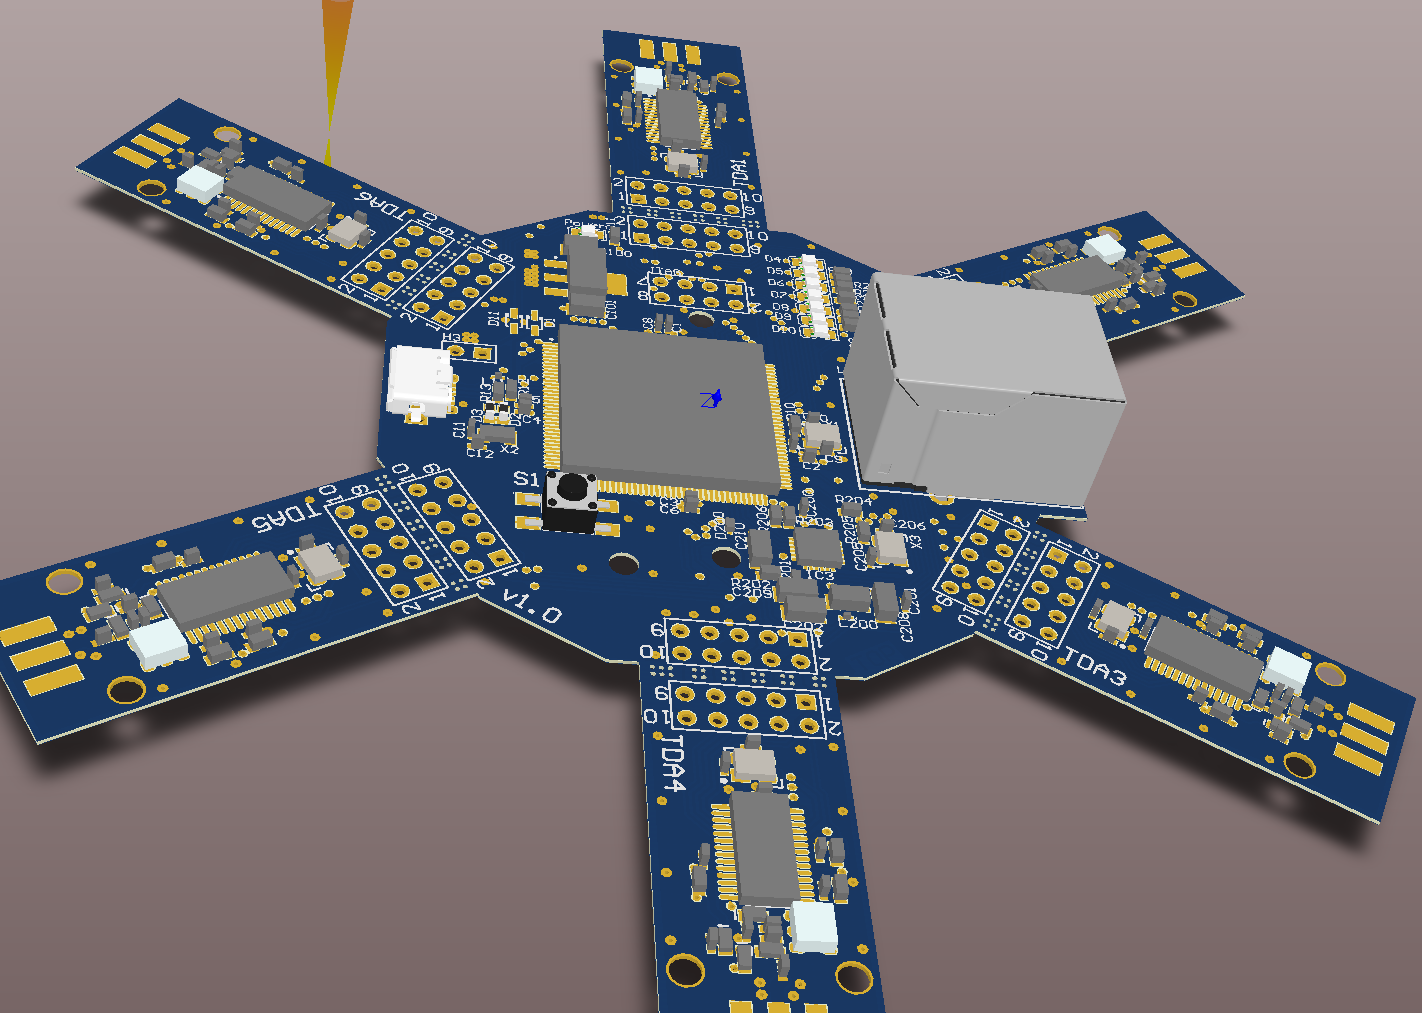
\includegraphics[width=\textwidth]{Abbildungen/Aufnahmen/Bilder/Altium/3D2}
	\caption{Layout des Aufsteckboards mit dem TDA5340}
	\label{fig:3D}
\end{figure}
\subsection{Gehäuse}
\label{app:Gehäuse}






\newpage
\section{Layout TDA5340 Aufsteckboard}
Das Layout der Transceiver-Unterbaugruppen orientiert sich an dem Layout eines Aufsteckboards für den \enquote{XMC 2Go} damit ein TDA5340 auf mit diesem verwendet werden kann. 

\begin{figure}[h] 
	\centering
	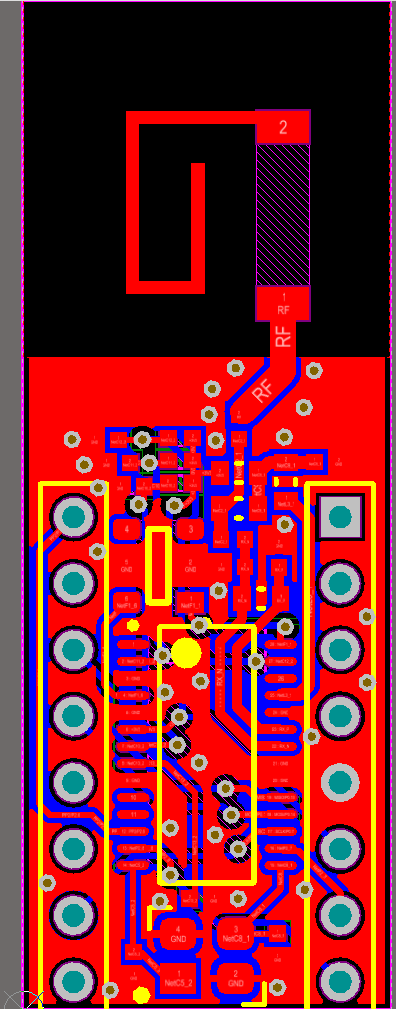
\includegraphics[height=\textwidth, angle=-90 ]{Abbildungen/Aufnahmen/Bilder/Altium/Layout_Stefan_Erhard/Layout.png}
	\caption{Layout des Aufsteckboards mit dem TDA5340}
	\label{fig:AufsteckboardTDA}
\end{figure}

\section{Quellcode}
\subsection{Main.c}
%\lstinputlisting[language=C]{../../Dave/Basisstation/Basisstation/Main.c}
\subsection{ISRs.c}
\lstinputlisting[language=C]{../../Dave/Basisstation/Basisstation/ISRs.c}
\subsection{Init.c}
\lstinputlisting[language=C]{../../Dave/Basisstation/Basisstation/Init.c}